%%%%%%%%%% CITIS-Final-Paper-Optimizacion-Finished.tex %%%%%%%%%%%%%%%%%%%%
%
%  Articulo final en la plantilla SNmult (Springer Nature, contributed
%  volume) solicitada para CITIS. Las seis estrategias (incluido ALNS con
%  resultados reales) estan completas; no quedan marcadores \todo{}
%  activos en el cuerpo (el macro se deja definido por si hace falta en
%  una revision futura).
%
%  LIMITE DE PAGINAS: CITIS exige 12-15 paginas INCLUYENDO figuras,
%  tablas y referencias. Esta version ocupa exactamente 15. Con las tres
%  figuras del benchmark ocupaba 16, asi que solo se conserva
%  figures/comparison_row_N200.png (la unica con contenido propio);
%  figures/scalability.pdf y figures/pareto_N400.pdf siguen en la carpeta
%  "figures/" y solo reproducen columnas de la Tabla 1. Si se recuperan,
%  hay que anadirlas tambien al fichero ALT_Text (una fila por figura).
% =====================================================================

\documentclass[graybox]{SNmult}

\usepackage{type1cm}
\usepackage{makeidx}
\usepackage{graphicx}
\usepackage{multicol}
\usepackage[bottom]{footmisc}
\usepackage{newtxtext}
\usepackage[varvw]{newtxmath}
\usepackage{amsmath}
\let\Bbbk\undefined % Resolves amssymb \Bbbk collision
\usepackage{amssymb}
\usepackage{booktabs}
\usepackage{algorithm}
\usepackage{algpseudocode}
\usepackage{url}
\usepackage{xcolor}

\makeindex             % como en la plantilla: usar el estilo svind.ist
                       % con su programa makeindex

% Marcador visible para pendientes de recalculo/edicion antes de enviar.
% Buscar "\todo{" en el fuente para ubicar todos los pendientes.
\newcommand{\todo}[1]{\textcolor{red}{\textbf{[PENDIENTE: #1]}}}

% Float parameters: the defaults reserve so much of each page for text
% that a half-page figure forces a near-empty page. Loosening them lets a
% figure share its page with a full column of text, which is what keeps
% the chapter inside the 15-page limit.
\renewcommand{\topfraction}{0.92}
\renewcommand{\bottomfraction}{0.75}
\renewcommand{\textfraction}{0.07}
\renewcommand{\floatpagefraction}{0.80}

\begin{document}
% \motto{...}   % opcional: la plantilla admite un motto por capitulo;
                % se deja sin usar salvo que los autores quieran uno.
\title*{Capacitated School Bus Routing via Clustering and
Network-Based Optimization: A Comparative Benchmark of Six Strategies
on a Real Road Network}
\titlerunning{Capacitated School Bus Routing: A Comparative Benchmark}

% --- Bloque de autoria camera-ready ---------------------------------
\author{Roy Sandoval\orcidID{0009-0009-0824-2390} \and
Sara R\'ua\orcidID{0009-0002-7170-7479} \and
Mariana Arbel\'aez\orcidID{0009-0005-3642-2760} \and
Naomi Chow\orcidID{0009-0003-0356-3167} \and
Daniel L\'opez\orcidID{0009-0001-9911-2904} \and
Roberto Hincapi\'e\orcidID{0000-0003-2525-1247}}
\authorrunning{Sandoval et al.}
% All six authors share one affiliation, so they are grouped under a
% single \at block rather than repeating the department, university, city
% and country six times. Every author still carries their institutional
% e-mail, as the camera-ready checklist requires.
\institute{\sloppy\emergencystretch=3em\relax Roy Sandoval, Sara R\'ua, Mariana Arbel\'aez, Naomi Chow,
Daniel L\'opez and Roberto Hincapi\'e \at Ingenier\'ia en Ciencia de
Datos, Universidad Pontificia Bolivariana, Medell\'in, Colombia.
e-mail: roy.sandoval@upb.edu.co, sara.ruag@upb.edu.co, mariana.arbelaezs@upb.edu.co, naomi.chow@upb.edu.co, daniel.lopezlo@upb.edu.co, roberto.hincapie@upb.edu.co}

\maketitle

\abstract*{The School Bus Routing Problem (SBRP) is an NP-hard
generalization of the capacitated vehicle routing problem, yet
head-to-head comparisons of its heuristics under identical conditions
remain scarce. We benchmark six strategies based on
clustering, set covering and adaptive search on identical scenarios from
the real OpenStreetMap road network of Medell\'in (Colombia). All share a solver interface, directed shortest
paths, a single depot and a capacity of twenty, and are measured on fleet
distance, computation time, coverage and cluster cohesion across
densities $N\in\{50,100,200,400\}$ with eleven seeds each (264 runs).
Under an identical wall-clock budget, Adaptive Large Neighborhood Search
(ALNS) achieves the shortest fleet distance at every density, winning all
44 scenarios against the clustering pipelines (mean rank 1.02 of 6) and
calibrating within 0.22\% of known CVRP optima. It yields those routes
with the \emph{least} cohesive clusters (silhouette 0.068 vs.\ 0.276 for
K-medoids at $N{=}400$), indicating that spatial compactness is a
byproduct of good routes, not their cause. The
zonal CVRPTW instead caps ride time, cutting the longest route by
30--47\% at $N{=}400$, while the two set-covering programs trade distance
for speed at
two different points because they optimize different objectives. We
distil these trade-offs into solver-selection guidance.
\keywords{School Bus Routing Problem $\cdot$ Capacitated clustering $\cdot$
Vehicle routing $\cdot$ Set covering $\cdot$ Road-network optimization.}}

\abstract{The School Bus Routing Problem (SBRP) is an NP-hard
generalization of the capacitated vehicle routing problem, yet
head-to-head comparisons of its heuristics under identical conditions
remain scarce. We benchmark six strategies based on
clustering, set covering and adaptive search on identical scenarios from
the real OpenStreetMap road network of Medell\'in (Colombia). All share a solver interface, directed shortest
paths, a single depot and a capacity of twenty, and are measured on fleet
distance, computation time, coverage and cluster cohesion across
densities $N\in\{50,100,200,400\}$ with eleven seeds each (264 runs).
Under an identical wall-clock budget, Adaptive Large Neighborhood Search
(ALNS) achieves the shortest fleet distance at every density, winning all
44 scenarios against the clustering pipelines (mean rank 1.02 of 6) and
calibrating within 0.22\% of known CVRP optima. It yields those routes
with the \emph{least} cohesive clusters (silhouette 0.068 vs.\ 0.276 for
K-medoids at $N{=}400$), indicating that spatial compactness is a
byproduct of good routes, not their cause. The
zonal CVRPTW instead caps ride time, cutting the longest route by
30--47\% at $N{=}400$, while the two set-covering programs trade distance
for speed at
two different points because they optimize different objectives. We
distil these trade-offs into solver-selection guidance.
\keywords{School Bus Routing Problem $\cdot$ Capacitated clustering $\cdot$
Vehicle routing $\cdot$ Set covering $\cdot$ Road-network optimization.}}

% =====================================================================
\section{Introduction}
% =====================================================================
The School Bus Routing Problem\index{School Bus Routing Problem} (SBRP)
plans a fleet of buses that collects students from a set of stops and
delivers them to their school under constraints such as vehicle capacity,
maximum riding time and bell-time windows~\cite{Park2010TheReview}. It
generalizes the capacitated vehicle routing problem, a descendant of the
truck-dispatching problem of Dantzig and
Ramser~\cite{DantzigRamser1959Truck}, and is NP-hard: a bus visiting $n_c$
stops admits $n_c!$ orders, and the partition across buses must be chosen
jointly with those orders. Practical solvers are therefore overwhelmingly
heuristic, and the surveys of Park and Kim~\cite{Park2010TheReview} and
Ellegood et al.~\cite{Ellegood2020SchoolDirections} show a field
fragmented into variants whose relative merits are rarely measured on
common ground.

Three families dominate. The \emph{cluster-first, route-second}\index{cluster-first, route-second}
paradigm groups students into capacity-feasible clusters and solves a
Traveling Salesman Problem (TSP) in each, using
2-opt~\cite{Croes1958TwoOpt} or Lin--Kernighan~\cite{HelsgaunAnHeuristic},
with clustering driven by geometry~\cite{CakirRevisitingProblem},
partitioning algorithms~\cite{Comert2018AStudy} or conflicting
objectives~\cite{Corberan2002HeuristicObjectives}. A second formulates
route selection as a set-covering\index{set covering} integer program; a
third uses metaheuristics~\cite{Baranwal2016DAVRPTW,Hatamlou2018BlackHole}.
Published on different instances, distance models, objectives and budgets,
their numbers cannot be compared directly. Our contributions are:

\begin{itemize}
\item A \textbf{unified benchmark harness} exposing six SBRP strategies
through one interface and evaluating them on \emph{identical} scenarios
built from the real road network of Medell\'in and the Valle de Aburr\'a,
under the same capacity, distance model and metrics.
\item A \textbf{rigorous description} of each strategy: a formal
decision-variable model and worst-case complexity checked against
\emph{measured} per-stage cost, making explicit where strategies that look
comparable optimize different objectives.
\item A \textbf{statistically grounded comparison} across four densities
and eleven seeds (264 runs) with Friedman, Wilcoxon and Nemenyi tests,
plus \textbf{external calibration} of the winning strategy against $27$
published CVRP instances with known optima (Section~\ref{sec:external}).
\item \textbf{Practical guidance}: an adaptive large-neighbourhood search
(ALNS, Section~\ref{sec:alns}) given the same wall clock as the clustering
pipelines returns the shortest fleet distance in every scenario, while
set-covering programs hold the speed end of the trade-off. It does so
with the \emph{least} cohesive clusters of the six, evidence that
compactness is a means to short routes, not a proxy for them
(Section~\ref{sec:discussion}).
\end{itemize}

\paragraph{Relevance to data-driven urban planning.}
This work addresses \emph{smart mobility and data-driven urban planning}:
it decides school transport from the real street topology of a
metropolitan area, and re-targets to another city by swapping the graph
and service polygons. Total fleet distance is exactly the
vehicle-kilometres travelled (VKT) that drives fuel use, emissions and
congestion, so the spread between solvers is not merely algorithmic. At
$N=400$ the worst strategy ($670$~km) commits $1.56\times$ the VKT of the
best ($428$~km) for the same students, buses and network, and the $32$~km
ALNS saves over the best clustering pipeline is $7\%$ of the daily fleet
distance recovered by changing solver alone. Converting VKT to emissions
needs fleet-specific factors we lack, so we stop
there~\cite{Sabet2022GreenVRP}.

% =====================================================================
\section{Related Work}\label{sec:related}
% =====================================================================
\subsection{The School Bus Routing Problem}
Park and Kim~\cite{Park2010TheReview} decompose the SBRP into five
sub-problems (data preparation, bus-stop selection, route generation,
route scheduling, bell-time adjustment) and observe that most work tackles
one or two in isolation. Over 64 later publications, Ellegood et
al.~\cite{Ellegood2020SchoolDirections} confirm single-school,
capacity-constrained route generation as the most studied core, dominated
by heuristics, while Wang et al.~\cite{Wang2025SBRPReview} record a shift
towards multi-objective and learning-based methods and name what motivates
this paper: the proliferation of variants has outpaced comparative
evaluation. Corber\'an et al.~\cite{Corberan2002HeuristicObjectives}
stress that minimizing buses and minimizing riding time conflict. We adopt
the single-school, capacitated, route-generation variant and report
several competing objectives side by side.

\subsection{Cluster-first, route-second}
Cakir et al.~\cite{CakirRevisitingProblem} revisit cluster-first,
route-second with a shape-based clustering that forms clusters of a
desired geometry relative to the depot, the conceptual ancestor of our
sectorial strategy. Comert et al.~\cite{Comert2018AStudy} partition
customers with k-means, k-medoids or random clustering before routing and
report medoid-based clustering as the most robust, which our results
corroborate on a real road network. The k-medoids/PAM family originates
with Kaufman and Rousseeuw~\cite{KaufmanRousseeuw1990PAM}; we use the
FasterPAM variant. The sub-trajectory set-cover formulation of Akitaya et
al.~\cite{Akitaya2021Subtrajectory} links the two paradigms we
contrast.

\subsection{Routing and metaheuristics}
Within a cluster, route construction reduces to the TSP, for which the
savings heuristic~\cite{ClarkeWright1964Savings}, 2-opt~\cite{Croes1958TwoOpt}
and Lin--Kernighan~\cite{HelsgaunAnHeuristic} are the classical tools.
Modern solvers wrap these in metaheuristics: OR-Tools~\cite{PerronFurnon2023ORTools},
which we use for the routing stage, drives local search with Guided Local
Search~\cite{Voudouris1999GLS}. Population- and physics-inspired
metaheuristics are widely applied to routing (deterministic
annealing~\cite{Baranwal2016DAVRPTW}, the black-hole
algorithm~\cite{Hatamlou2018BlackHole}, genetic
algorithms~\cite{Holland1992Adaptation}), and learning-based approaches
have matured from graph convolutional
networks~\cite{Joshi2019GCN,Dahiya2018TSPReview} into a distinct family of
neural VRP solvers~\cite{Wu2024NCOSurvey}, alongside emissions-aware
``green'' VRP variants~\cite{Sabet2022GreenVRP}. Adaptive
large-neighbourhood search enters our benchmark as the locality-aware
representative of that family (Section~\ref{sec:alns}), though one
configuration does not bound it.

% =====================================================================
\section{Methods}\label{sec:methods}
% =====================================================================
This section presents the methods in three parts: the formal problem
statement (Section~\ref{sec:problem}), the six solution strategies
with their models and complexity, including the adaptive
large-neighbourhood search (ALNS)
(Sections~\ref{sec:framework}--\ref{sec:alns}), and the experimental
protocol (Section~\ref{sec:setup}).

\subsection{Problem formulation}\label{sec:problem}
\subsubsection{Notation and distances.}
Let the road network be a directed weighted graph $G=(V,E)$ with arc
weights $w_e>0$, a single school (depot) $o\in V$, $n$ student stops
$\mathcal{C}=\{1,\dots,n\}\subset V$ and a homogeneous fleet of capacity
$C$. The road distance $d_{ij}$ is the shortest-path cost
$\min_{p\in\mathcal{P}(i,j)}\sum_{e\in p} w_e$ over directed paths, and is
in general asymmetric ($d_{ij}\neq d_{ji}$). Clustering algorithms that
assume a metric use the symmetrized
$D^{\mathrm{sym}}_{ij}=\tfrac{1}{2}(d_{ij}+d_{ji})$; the routing stage
uses the directed $d_{ij}$.

\subsubsection{Objective and constraints.}
The SBRP we address is a single-depot CVRP. A solution is a set of closed
routes, one per bus, each starting and ending at $o$; the number of buses
is lower-bounded by $k=\lceil n/C\rceil$. The objective minimizes total
fleet distance
\begin{equation}
L_{\mathrm{total}}=\sum_{c}\sum_{(i,j)\in r_c} d_{ij}\,,
\label{eq:obj}
\end{equation}
subject to: (i)~every student is served by exactly one bus (full
coverage); (ii)~no route carries more than $C$ students; and
(iii)~every route starts and ends at the depot. Because solving this
CVRP exactly is intractable, we adopt the cluster-first, route-second
decomposition into a capacitated assignment sub-problem followed by
$k$ independent TSPs.

Constraint~(i) is hard for five of the six strategies, including ALNS,
which repairs every destroyed solution back to full coverage before it is
accepted. The zonal CVRPTW is the exception: its route-duration limit can
conflict with coverage on peripheral stops, so it relaxes~(i) to
$\sum_{c} x_{ic}+u_i=1$ with $u_i\in\{0,1\}$ marking student $i$
unserved and adds $\Pi\sum_i u_i$ to the objective, $\Pi$ being large
enough that a drop costs more than any feasible detour
(Section~\ref{sec:cvrptw}). Coverage is a first-class metric, so this
relaxation stays visible in every comparison.

\subsubsection{Capacitated assignment sub-problem.}
Given current cluster representatives (medoids)
$M=\{m_1,\dots,m_k\}$, the assignment of students to clusters is the
binary program
\begin{align}
\min\; \sum_{i,c} D^{\mathrm{sym}}_{i,m_c}\,x_{ic}
\;\;\text{s.t.}\;\; & \textstyle\sum_{c} x_{ic}=1\;\;\forall i,
\label{eq:assign-obj}\\
& \textstyle\sum_{i} x_{ic}\le C\;\;\forall c,\quad x_{ic}\in\{0,1\},
\label{eq:assign-cap}
\end{align}
where $x_{ic}=1$ iff student $i$ joins cluster $c$. Its constraint matrix
being totally unimodular, the program is solved to optimality as a
minimum-cost flow in a four-layer network (source $\to$ students $\to$
medoids $\to$ sink), avoiding a general integer solver. Each medoid is
then recomputed as the within-cluster $1$-median $m_c=\arg\min_{h\in
S_c}\sum_{i\in S_c} D^{\mathrm{sym}}_{ih}$, and the two steps alternate
until the medoids stabilize.

\subsubsection{Per-cluster routing sub-problem.}
For cluster $c$ with node set $V_c=S_c\cup\{o\}$ and binary arc variables
$y_{ij}$, the route is the TSP tour minimising
$\sum_{(i,j)} d_{ij}y_{ij}$ subject to unit in- and out-degree at every
node and the Dantzig--Fulkerson--Johnson subtour-elimination family
\begin{equation}
\textstyle\sum_{i\in S}\sum_{j\in S} y_{ij}\le |S|-1
  \quad \forall\, S\subsetneq V_c,\; 2\le|S|\le|V_c|-1,
  \label{eq:dfj}
\end{equation}
which rules out cycles that do not span $V_c$. Having exponentially many
members it is not enumerated: OR-Tools maintains a single connected
circuit by construction and improves it with Guided Local
Search~\cite{Voudouris1999GLS} under a fixed budget, so (\ref{eq:dfj})
defines the optimum we approximate, not the algorithm.

\subsubsection{Set-covering formulation.}\label{sec:setcover-formulation}
An alternative that bypasses explicit clustering enumerates a pool
$\mathcal{R}$ of capacity-feasible candidate routes and selects a
subset. Minimizing the number of buses gives the set-cover program
\begin{equation}
\min \sum_{j\in\mathcal{R}} x_j \quad\text{s.t.}\quad
\sum_{j:\,i\in R_j} x_j \ge 1\;\;\forall i\in\mathcal{C},\quad
x_j\in\{0,1\},
\label{eq:setcover}
\end{equation}
while replacing the objective by $\sum_j \mathrm{cost}_j\,x_j$ (the
route length) minimizes distance instead. Both variants are solved
with a branch-and-cut integer solver. That objective choice is not
incidental: our two set-covering strategies instantiate different sides of
Eq.~(\ref{eq:setcover}), so comparing them on distance alone mixes pool
construction with objective choice (Section~\ref{sec:setcover-two}).

\subsection{Common benchmark framework}\label{sec:framework}
All strategies are adapters behind one \texttt{Solver} interface: each
receives a \texttt{Scenario} (the same road graph, student locations,
depot and capacity) and returns a \texttt{Solution} (closed routes and,
optionally, cluster labels), so all are evaluated on byte-identical inputs
and scored by identical metric code. It uses
OSMnx~\cite{Boeing2017OSMnx} for network extraction, NetworkX for graph
algorithms and minimum-cost flow, OR-Tools~\cite{PerronFurnon2023ORTools}
for TSP/CVRPTW search, FasterPAM~\cite{KaufmanRousseeuw1990PAM} for medoid
initialization, CBC for the set-covering programs and
scikit-learn~\cite{Pedregosa2011Sklearn} for the silhouette score, and is
deterministic given $(N,\text{seed})$. This interface is what lets the
ALNS adapter enter the comparison without touching the scenarios or any
other strategy.

\subsection{Capacitated k-medoids + OR-Tools (baseline)}
The baseline instantiates the cluster-first, route-second decomposition as
formalized above: FasterPAM provides initial medoids, the capacitated
assignment of Eqs.~(\ref{eq:assign-obj})--(\ref{eq:assign-cap}) is solved
by minimum-cost flow, medoids are recomputed as within-cluster
$1$-medians, and the loop iterates to convergence or a cap $T$ before each
cluster is routed with OR-Tools.

\subsection{Sectorial multi-objective clustering}
The sectorial strategy replaces the distance-driven assignment with a
geometric one inspired by shape-based
clustering~\cite{CakirRevisitingProblem}, scoring each student by a convex
combination of angular position and radial distance from the school,
\begin{equation}
s_i=\alpha\,\frac{\theta_i+\pi}{2\pi}+\beta\,\hat d_i,
\qquad \alpha+\beta=1,
\label{eq:sectorial-score}
\end{equation}
with $\theta_i=\operatorname{atan2}(y_i-y_o,\,x_i-x_o)$ and $\hat d_i$ the
min--max-normalized depot distance ($\alpha=0.6,\beta=0.4$). An angular
sweep packs students into capacity-bounded sectors, refined by the
baseline's minimum-cost-flow reassignment, giving compact wedge-shaped
clusters radiating from the school.

\subsection{Zonal CVRPTW}\label{sec:cvrptw}
This strategy partitions the metropolitan area into six fixed zones
(communes and municipalities of the Valle de Aburr\'a, by
point-in-polygon test) and solves an independent CVRPTW per zone with
OR-Tools. Beyond capacity it enforces a time dimension: travel time plus
$90$~s boarding per stop, a $75$-minute maximum route duration and a
span-balancing penalty. Unserved stops are allowed at high penalty, so a
small fraction of students can be left uncovered when the limit binds.

Formally, with $Z$ indexing zones, $\mathcal{C}_z$ the students inside
zone $z$, binary arc variables $y^z_{ij}$, drop indicators
$u_i\in\{0,1\}$ and arrival times $a_i\ge0$, each zone solves
\begin{equation}
\min \sum_{z\in Z}\big[\sum_{(i,j)} d_{ij}y^z_{ij} + \gamma\sigma_z\big]
 + \Pi\sum_{i\in\mathcal{C}} u_i
,\ \text{s.t.}\, \textstyle\sum_{j} y^z_{ij} = 1-u_i,\,
\sum_{i\in r} q_i \le C,\, a_j \ge a_i + \tau_{ij} + b
\label{eq:cvrptw}
\end{equation}
plus $a_{\text{end}}-a_{\text{start}}\le T_{\max}$ per route, with
$\tau_{ij}$ directed travel time, $b=90$~s boarding, $T_{\max}=75$~min,
$\sigma_z$ the duration span penalized by $\gamma$, and $\Pi$ the drop
penalty of Section~\ref{sec:problem}. The constraint
$\sum_j y^z_{ij}=1-u_i$ is the soft-coverage relaxation: a student is
visited once or dropped at cost $\Pi$, and since $\Pi$ dominates any
routing saving, drops arise only where the duration limit admits no
feasible insertion. With a single bell time the time windows reduce to
that limit, which is what binds here.

\subsection{Set-covering integer programs}\label{sec:setcover-two}
Two variants instantiate Eq.~(\ref{eq:setcover}) \emph{differently},
building different candidate pools and optimizing different objectives, so
they are two policies rather than two implementations of one. The
\emph{per-child} variant builds
$\mathcal{R}=\{R_1,\dots,R_n\}$ with $R_i=\{i\}\cup\mathrm{NN}_{C-1}(i)$,
the $C-1$ nearest neighbours of $i$ under $D^{\mathrm{sym}}$, giving $n$
candidates in $O(n^2)$ time, and minimizes $\sum_j x_j$, i.e.\ fleet size.
The \emph{grid} variant overlays a Cartesian lattice whose spacing shrinks
with student density, greedily grows one capacity-feasible route around
each occupied cell's seed, and minimizes
$\sum_j \mathrm{cost}_j x_j$ with $\mathrm{cost}_j$ the length of a greedy
tour over $R_j$, i.e.\ distance directly. Both are solved by
branch-and-cut.

Because per-child never receives a distance term, its routes are the
cheapest-in-fleet-size candidate it was asked for, not a
distance-minimizing one that lost, so reading its longer routes as a
quality gap needs care; three factors contribute and our design separates
none. Eq.~(\ref{eq:setcover}) is a \emph{covering} ($\ge1$) rather than
\emph{partitioning} ($=1$) constraint and routes run as generated, so a
student in two selected candidates is visited twice and both visits are
charged: at $N=400$ per-child selects $26.9$ capacity-filled routes, $538$
seats for $400$ students, about a quarter of visits redundant.
$\mathcal{R}$ is also a heuristically seeded subset of all
$\binom{n}{\le C}$ feasible routes, so branch-and-cut speed reflects a
small pool rather than an easy program. And the objectives differ, so
comparing the two on distance conflates pool quality with objective
choice; isolating pool construction would mean running each objective on
the other's pool, left to future work.

\subsection{Adaptive large-neighbourhood search}\label{sec:alns}
\index{adaptive large-neighbourhood search (ALNS)}
The five strategies above cover cluster-first, route-second pipelines and
set-covering programs; ALNS adds a locality-aware metaheuristic behind the
same \texttt{Solver} interface, measured on the same scenarios and
metrics. It starts from a feasible solution and repeatedly \emph{destroys} and
\emph{repairs} part of it. A destroy operator removes a subset of
students, drawn from a pool of random removal,
worst-cost removal (students whose removal shortens their route most) and
Shaw-style related removal (students close in $D^{\mathrm{sym}}$ or
sharing a route, so removing them together opens a genuinely new
neighbourhood). A repair operator reinserts them by cheapest feasible
insertion or a regret-$k$ criterion that anticipates future insertion
cost, respecting Eq.~(\ref{eq:assign-cap}) at every step. Each iteration
picks one operator of each kind, evaluates the result against
$L_{\mathrm{total}}$ (Eq.~\ref{eq:obj}) and accepts or rejects it under a
simulated-annealing criterion, so the search can escape local optima
without discarding the structure cluster-first, route-second exploits.
Operator weights are updated adaptively from recent success, the property
that names the method and that lets it recover the locality a
topology-agnostic representation lacks.

\paragraph{Parameters and budget.}
The search is \emph{budget-matched} to the clustering pipelines: an
instance gets $B_{\mathrm{A}}=k\cdot B$ seconds of wall clock with
$B=5$~s, exactly the per-cluster TSP budget K-medoids and Sectorial spend
inside OR-Tools, so $15$, $25$, $50$ and $100$~s at $N=50,100,200,400$.
Any quality difference is therefore attributable to the search, not to
compute. The initial solution must accordingly be cheap: it reuses the
baseline's capacitated k-medoids partition
(Eqs.~(\ref{eq:assign-obj})--(\ref{eq:assign-cap})) but routes each
cluster with a nearest-neighbour tour plus 2-opt rather than calling
OR-Tools, costing $\le1.1\%$ of the budget and leaving $10$k--$15$k
destroy--repair iterations.

Each iteration removes $q\sim\mathcal{U}[0.10n,\,0.25n]$ students, capped
at $60$. Worst- and Shaw-removal pick from their ranked candidate lists
with the randomisation $L[\lfloor |L|\cdot y^{p}\rfloor]$,
$y\sim\mathcal{U}(0,1)$, $p=3$, so the choice is greedy but not
deterministic. Operator weights start at $w_\omega=1$ and update as
$w_\omega \gets \theta w_\omega + (1-\theta)s_j$ with reaction factor
$\theta=0.8$ and scores $(5,2,1,0.5)$ for a new global best, an
improvement, an accepted solution and a rejected one. Acceptance is
simulated annealing with geometric cooling $T_t=T_0\gamma^{\,t}$, $T_0$
fitted so a solution $5\%$ worse than $r_0$ is accepted with probability
$0.5$ initially and $\gamma$ annealing to $T=1$ over a $25{,}000$-iteration
horizon. All values are fixed across the sweep, with no per-instance
tuning, as for the other five strategies (Sec.~\ref{sec:setup}).

\subsection{Complexity analysis}\label{sec:complexity}
Asymptotically, the two flow-based pipelines cost $O(T\,n^3)$ (min-cost
flow), the zonal CVRPTW $O(n^2)$--$O(n^3)$ under Guided Local Search, the
set-covering variants an exponential ILP over an $O(n^2)$ or $O(n)$ pool,
and ALNS $O(I\,n)$--$O(I\,n\log n)$ ($n$ students, $k=\lceil n/C\rceil$
buses, $T$ the iteration cap). Those bounds do not govern wall-clock time,
so we timed the stages instead. For K-medoids and Sectorial the
minimum-cost-flow assignment takes $0.04\%$ of solver time at $N=50$ and
$1.1\%$ at $N=400$ ($1.09$ of $101.13$~s), FasterPAM under $0.02$~s; the
per-cluster TSP takes the rest and is \emph{budget-bound}, costing almost
exactly $k\cdot B$ ($15.03$, $25.01$, $50.01$, $100.03$~s for
$k=3,5,10,20$), so latency grows linearly in $n$ and the $O(T\,n^3)$ bound
stays latent. ALNS is budget-bound by construction, so its timers answer
how many iterations the budget buys: repair takes $65$--$71\%$ of a run
against $17$--$29\%$ for destroy, since each insertion is scored over
every route and position, an $O(k\,|r|)$ sweep per removed student,
whereas removal needs one pass. Initial construction never exceeds
$1.1\%$, and the realised iteration count falls only from $15{,}095$ to
$10{,}353$ as $n$ grows eightfold.

\subsection{Experimental setup}\label{sec:setup}
Scenarios are generated on the real drivable road network of Medell\'in
and the Valle de Aburr\'a, extracted from OpenStreetMap with
OSMnx~\cite{Boeing2017OSMnx} and restricted to the largest strongly
connected component. The depot is fixed at a university campus and $N$
stops are sampled uniformly from graph nodes inside the union of the six
service-zone polygons, so every instance stays within the metropolitan
footprint. Directed distance and travel-time matrices are precomputed with
Dijkstra's algorithm; bus capacity is $C=20$. We sweep $N\in\{50,100,200,400\}$ with eleven seeds each, giving $44$
scenarios and $264$ runs, recording fleet distance, wall-clock latency,
buses used, coverage, the silhouette
coefficient~\cite{Rousseeuw1987Silhouettes} on the symmetrized distances,
capacity violations and the longest single route. To keep latency
comparable the per-cluster TSP is capped at $5$~s and the per-zone CVRPTW
at $20$~s. All strategies run at fixed settings with no per-instance
tuning: K-medoids $T=50$; Sectorial $\alpha=0.6$, $\beta=0.4$, $T=5$; the
zonal CVRPTW $75$~min maximum duration, $90$~s boarding, span coefficient
$300$; ALNS the parameters of Section~\ref{sec:alns} under its matched
$k\cdot5$~s budget. Significance is assessed with the Friedman test
(blocks $=$ the $44$ scenarios) and pairwise differences with Wilcoxon
signed-rank.

\subsubsection{External calibration.}\label{sec:external}
Six in-house implementations on self-generated instances establish
relative standings but say nothing about absolute quality. We therefore
run the ALNS solver unchanged, through the same \texttt{Solver} interface,
on the $27$ instances of Augerat set~A~\cite{Augerat1995CVRP}, a classical
CVRP family with published optima, $n=31$ to $79$, capacity $100$. The loader reproduces the
TSPLIB \texttt{EUC\_2D} convention, integer
$\mathrm{nint}(\sqrt{\Delta x^2+\Delta y^2})$, verified by recomputing
each published optimal solution under our matrix and recovering its cost
for all $27$. These instances carry non-unit demands $q_i$, so capacity is
a demand sum rather than a stop count, and each declares a vehicle count
$\lceil \sum_i q_i / C\rceil$, so ALNS optimizes over the fleet size the
optimum uses. Each gets $60$~s. Only ALNS is run: the clustering pipelines
assume unit demand, under which their assignment is an exact minimum-cost
flow, and generalising them would change the algorithms compared.

% =====================================================================
\section{Results}\label{sec:results}
% =====================================================================
Table~\ref{tab:fleet} reports fleet distance and latency, generated
mechanically from the run output, and Figure~\ref{fig:pareto} plots the
two jointly at $N{=}400$. At the most demanding density
($N=400$), the remaining quality metrics (buses / coverage / silhouette /
longest route in km, means over $11$ seeds) are: K-medoids
$20.0/1.000/0.276/46.2$; Sectorial $20.0/1.000/0.266/45.2$; zonal CVRPTW
$22.4/0.998/0.272/30.3$; Set Cover per-child $26.9/1.000/0.230/50.8$; Set
Cover grid $23.2/1.000/0.199/56.6$; and ALNS $20.0/1.000/0.068/43.3$.
Every strategy but the zonal CVRPTW serves all students, and only the
covering programs exceed the minimum fleet of $k=\lceil n/C\rceil=20$
buses.

\begin{table}[tbp]
\centering
\caption{Total fleet distance (km, mean $\pm$ std over 11 seeds) and
latency (s, mean). Bold: distance minimum among full-coverage methods.}
\label{tab:fleet}
\setlength{\tabcolsep}{2pt}
\scriptsize
\begin{tabular}{l@{\hskip 5pt}rrrr@{\hskip 9pt}rrrr}
\toprule
& \multicolumn{4}{c@{\hskip 9pt}}{\textbf{Fleet distance (km)}}
& \multicolumn{4}{c}{\textbf{Latency (s)}}\\
\cmidrule(r){2-5}\cmidrule{6-9}
\textbf{Strategy} & $50$ & $100$ & $200$ & $400$ & $50$ & $100$ & $200$ & $400$\\
\midrule
K-medoids + TSP & 105$\pm$5 & 163$\pm$18 & 271$\pm$21 & 460$\pm$26 & 15.0 & 25.0 & 50.2 & 101.0 \\
Sectorial & 105$\pm$5 & 165$\pm$19 & 272$\pm$21 & 461$\pm$25 & 15.0 & 25.0 & 50.2 & 101.0 \\
CVRPTW (zonal)$^\ast$ & 125$\pm$7 & 182$\pm$12 & 286$\pm$16 & 471$\pm$13 & 100.0 & 100.0 & 100.0 & 100.0 \\
Set Cover (per-child) & 160$\pm$27 & 254$\pm$36 & 389$\pm$39 & 670$\pm$20 & 0.02 & 0.02 & 0.04 & 0.16 \\
Set Cover (grid) & 134$\pm$8 & 217$\pm$22 & 349$\pm$26 & 594$\pm$33 & 0.27 & 0.74 & 3.19 & 66.6 \\
ALNS & \textbf{98$\pm$5} & \textbf{155$\pm$19} & \textbf{251$\pm$19} & \textbf{428$\pm$24} & 15.0 & 25.0 & 50.0 & 100.0 \\
\bottomrule
\end{tabular}
\\[3pt]
{\footnotesize $^\ast$ CVRPTW may leave ${\sim}1\%$ of students unserved
when the duration limit binds, so its distance is not strictly comparable
to the full-coverage methods.}
\end{table}

\begin{figure}[tbp]
\centering
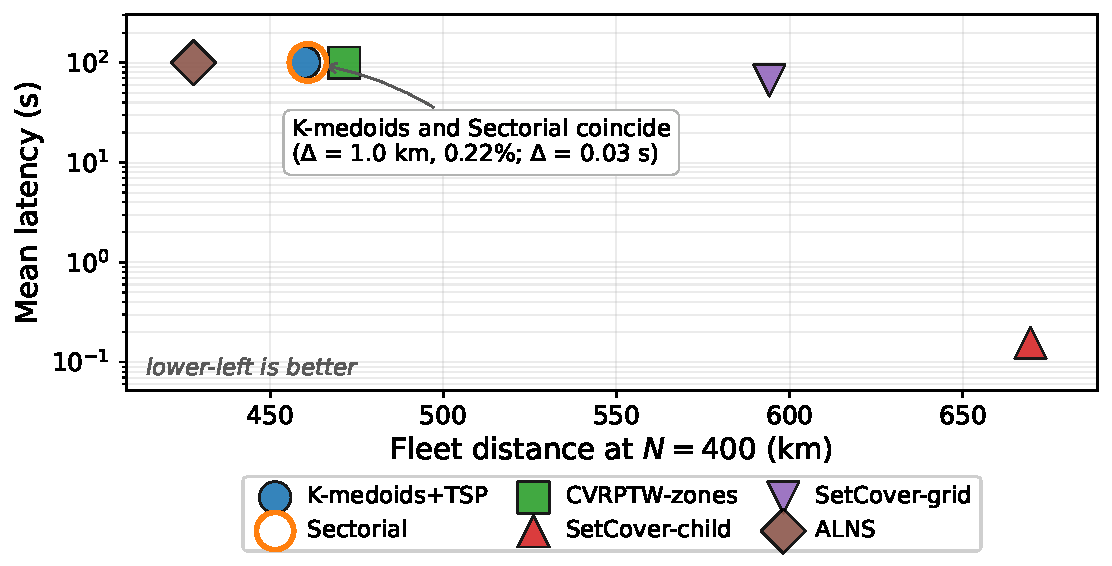
\includegraphics[width=0.54\textwidth]{figures/pareto_N400.pdf}
\Description{Scatter plot of fleet distance against mean latency at
N=400, one marker per strategy. ALNS sits furthest left (shortest
distance) at a latency matching the clustering pipelines; the two
set-covering variants sit far to the right on distance but far below on
latency; K-medoids and Sectorial are drawn as coincident markers.}
\caption{Fleet distance vs.\ latency at $N{=}400$ (lower-left is better).
Within the clustering pipelines' own budget, ALNS reaches the shortest
distance of the six; the set-covering variants trade distance for speed at
two different points; K-medoids and Sectorial are indistinguishable.}
\label{fig:pareto}
\end{figure}

\paragraph{Statistical significance.}
The Friedman test rejects equal performance across the six strategies for
both fleet distance ($\chi^2=201.74$, $\mathrm{df}=5$, $p<10^{-40}$) and
latency ($\chi^2=187.57$, $\mathrm{df}=5$, $p<10^{-37}$). On distance the
mean ranks (1 = best) are $1.02$ ALNS, $2.63$ Sectorial, $2.67$ K-medoids,
$3.68$ CVRPTW, $5.05$ Set Cover (grid) and $5.95$ Set Cover (per-child).
ALNS's $1.02$ reflects an almost unbroken sweep: it is shortest in $44$ of
$44$ scenarios against both clustering pipelines and $43$ of $44$ against
the zonal CVRPTW, whose single win comes on an instance where it leaves
students unserved. The two clustering leaders remain indistinguishable
from each other (Wilcoxon $p=0.36$), unaffected by which other strategies
are included. On latency Set Cover (per-child) is fastest in every
scenario (rank $1.00$), then Set Cover (grid) ($2.18$) and ALNS ($2.98$),
ahead of K-medoids ($4.59$), Sectorial ($4.82$) and CVRPTW ($5.43$). ALNS
outranking the clustering pipelines there is an artefact rather than a
speed advantage: all three get the same $k\cdot5$~s, but ALNS stops
exactly on budget whereas the OR-Tools calls overshoot by about $1\%$.

Since a Friedman rejection only says \emph{some} strategies differ, we add
the Nemenyi post-hoc~\cite{Demsar2006Statistical}, which separates two
strategies when their mean ranks differ by more than
$\mathrm{CD}=q_\alpha\sqrt{k(k+1)/6N}$; with $k=6$, $N=44$ and
$\alpha=0.05$ ($q_\alpha=2.850$), $\mathrm{CD}\approx1.14$. Of the
$\binom{6}{2}=15$ pairs, $11$ clear it on fleet distance. ALNS separates
from every other strategy: Set Cover (per-child) $\Delta=4.93$, Set
Cover (grid) $4.02$, zonal CVRPTW $2.66$ and, decisively for the headline
claim, K-medoids $1.65$ and Sectorial $1.60$. The clustering pipelines in
turn separate from Set Cover (per-child) ($3.28$--$3.33$) and Set Cover
(grid) ($2.38$--$2.42$), and the CVRPTW from both covering variants
($1.36$, $2.27$). Four pairs remain unresolved: K-medoids versus Sectorial
($0.045$), each against the CVRPTW ($1.01$--$1.06$), and the two covering
variants against each other ($0.91$). The design therefore resolves the
comparison that matters most, ALNS against the previous leaders, while
leaving the near-ties eleven seeds could not separate before.

\paragraph{Absolute quality against published optima.}
On the external instances of Section~\ref{sec:external} the same ALNS
configuration solves $19$ of the $27$ to proven optimality and averages
$0.221\%$ above the optimum, median gap exactly $0$; every solution is
capacity-feasible, covers all customers and uses the declared vehicle
count. The eight it does not close are the larger ones ($n\ge52$):
A-n61-k9 $0.10\%$, A-n63-k10 $0.38\%$, A-n60-k9 $0.66\%$, A-n63-k9
$0.68\%$, A-n53-k7 $0.69\%$, A-n69-k9 $0.78\%$, A-n80-k10 $0.96\%$ and
A-n64-k9 $1.71\%$. These are not a budget artefact: raising the limit to
$300$~s multiplies the iteration count sevenfold ($51.6$k to $360.2$k) yet
moves the mean gap only to $0.205\%$, leaving seven of the eight unchanged
and the proven optima at $19$. What remains is a limit of the operator
pool, not of the time given to it. Dedicated solvers close set~A routinely, so this does
not make our ALNS state-of-the-art, but it bounds what the rest of the
paper leaves open: the strategy that wins our benchmark is within a
fraction of a percent of optimal on independent instances, so the margins
in Table~\ref{tab:fleet} separate a near-optimal method from the rest
rather than six equally unvalidated ones.

% =====================================================================
\section{Discussion}\label{sec:discussion}
% =====================================================================
\paragraph{Clustering is a good heuristic, not the objective.}
Among the cluster-first, route-second pipelines the story is the familiar
one: K-medoids and Sectorial build compact, well-separated clusters,
K-medoids attaining the highest silhouette at $N=400$ ($0.276$), and
compactness shortens the inter-stop distances the per-cluster TSP must
traverse, so a good partition does most of the optimization before routing
begins~\cite{CakirRevisitingProblem,Comert2018AStudy}. The cheap angular
score (Eq.~\ref{eq:sectorial-score}) recovers essentially the quality of
medoid optimization (Wilcoxon $p=0.36$); Figure~\ref{fig:grid} puts
that geometry beside the two alternatives on a single scenario.

\begin{figure}[tbp]
\centering
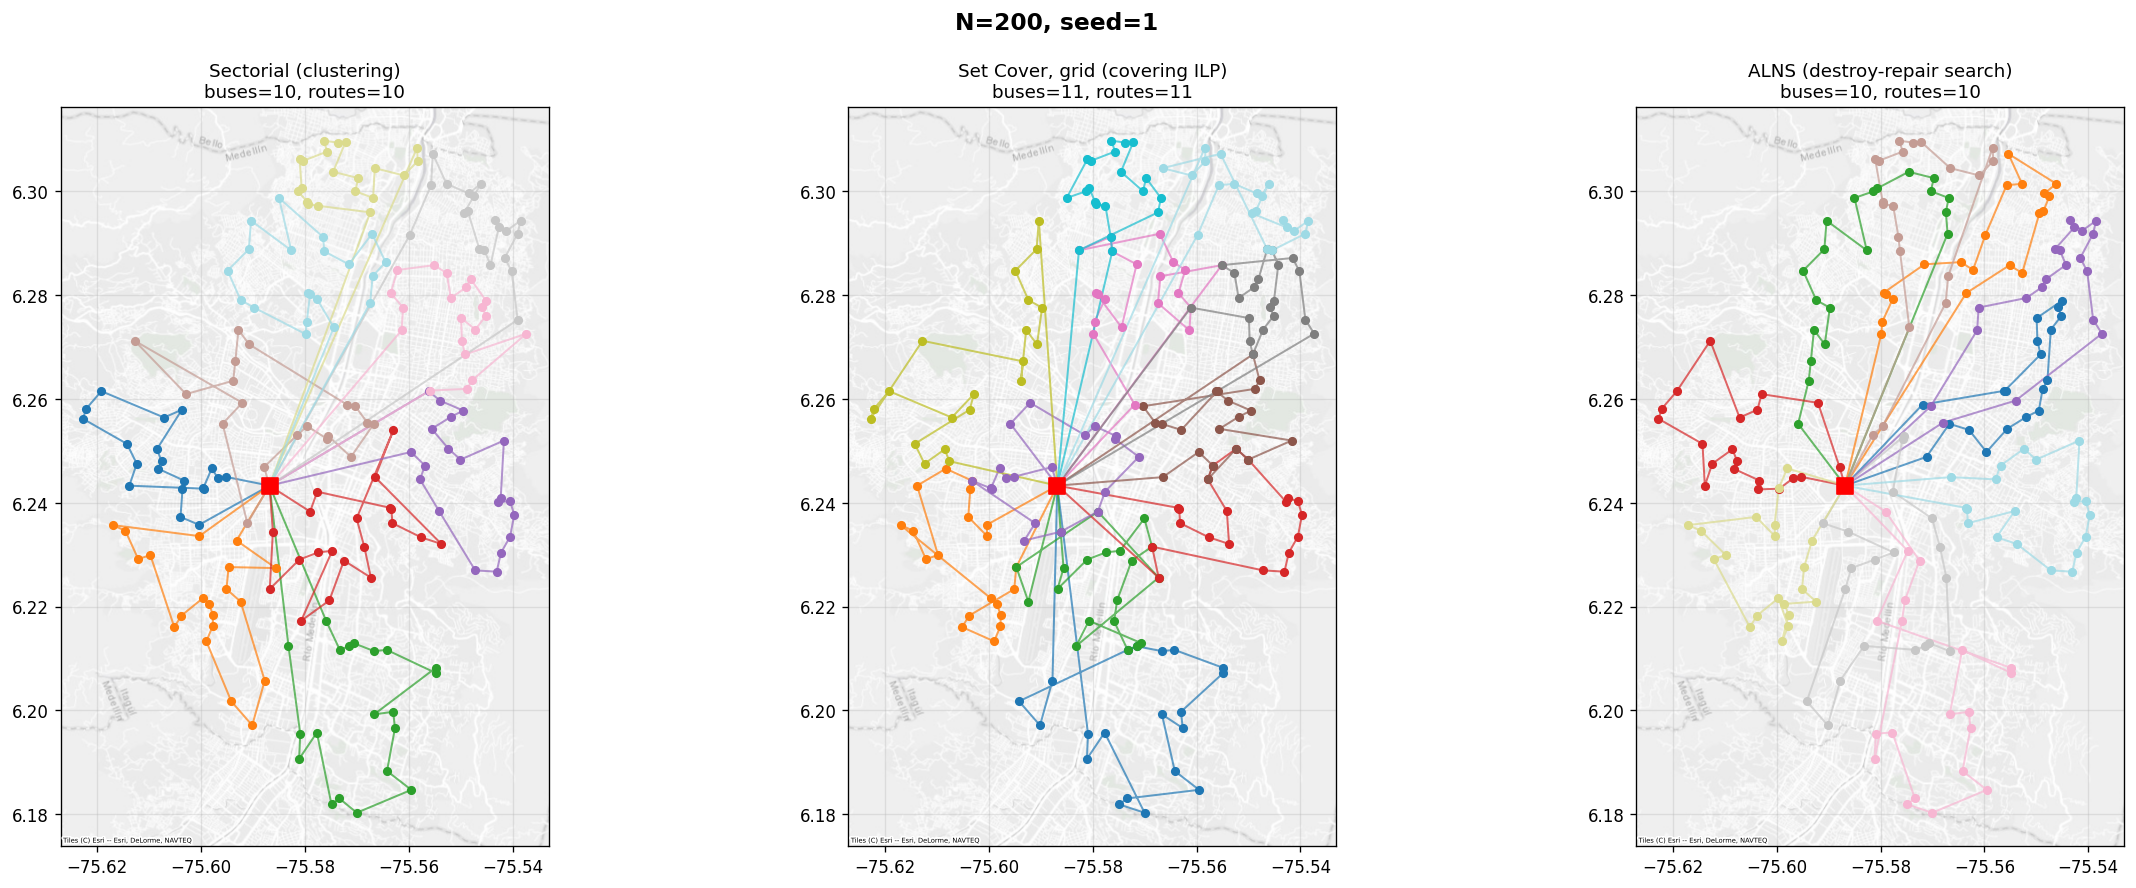
\includegraphics[width=0.66\textwidth]{figures/comparison_row_N200.png}
\Description{Three maps of the same N=200, seed 1 scenario over the
real Medellin road network. Left: Sectorial produces ten compact,
wedge-shaped clusters radiating from the depot. Centre: the grid
set-covering ILP selects eleven routes that overlap near the depot.
Right: ALNS produces ten routes, using the same fleet size as
Sectorial but with less visually compact, more interleaved routes.}
\caption{Three of the six strategies on one scenario ($N{=}200$, seed 1).
Left: Sectorial's wedge-shaped clusters. Centre: the grid set-covering
ILP, whose routes overlap near the depot because Eq.~(\ref{eq:setcover})
requires coverage, not a partition, and needs one more bus (11 vs.\ 10).
Right: ALNS, matching Sectorial's fleet size with a visibly less compact
partition.}
\label{fig:grid}
\end{figure}

ALNS breaks that story, and this is the most consequential finding here.
It attains the \emph{shortest} fleet distance at every density with by far
the \emph{least} cohesive partition: silhouette $0.068$ at $N=400$, a
quarter of K-medoids', falling monotonically with scale ($0.325$, $0.265$,
$0.174$, $0.068$) even as its advantage holds at $4.8$--$7.3\%$. A compact
partition is a good \emph{heuristic} for short routes because it makes
each TSP easy, but it is also a constraint, and a search optimizing
$L_{\mathrm{total}}$ directly spends that compactness whenever
interleaving two buses' territories buys a shorter tour. This also revises
the cohesion--cost correlation: at $N{=}400$ silhouette and fleet distance
correlate at $r=-0.95$ when the sixth strategy is a flat-permutation
genetic algorithm, as in an earlier iteration of this benchmark, but with
ALNS in its place the same computation gives $r=+0.09$ ($p=0.48$), and no
density shows a significant negative association. It was carried by one
strategy that was at once incoherent and long, not by a law relating the
two, so we report cohesion as descriptive rather than predictive.

\paragraph{The CVRPTW trade-off.}
The zonal CVRPTW yields competitive distances but is not free: it leaves
up to ${\sim}1\%$ of students unserved when the $75$-minute duration limit
binds and uses more buses than the optimum ($22.4$ vs.\ $20$ at $N=400$).
In exchange it produces by far the most \emph{balanced} routes: its
longest route ($30.3$~km) is $30$--$47\%$ shorter than any other method's,
because the span-balancing penalty and the explicit time dimension cap
individual ride times. Where bounded ride time is a hard requirement, it
is the only strategy that delivers it directly.

\paragraph{Set covering: speed, at two different objectives.}
The set-cover programs are the speed champions, per-child solving every
instance in under a quarter of a second and grid an order of magnitude
slower but still far faster than the clustering pipelines at $N\le200$. On
distance they take the last two places (mean ranks $5.05$ and $5.95$); on
latency the first two ($2.18$ and $1.00$). Their route quality should not
be compared with each other, however, for the reasons of
Section~\ref{sec:setcover-two}: they optimize different objectives over
differently built pools, so the gap mixes two effects. Grid's latency also
turns erratic at $N=400$ ($66.6\pm34.7$~s) as the pool, and hence the
integer program, grows. Both remain right when a feasible plan is needed
in near-real-time.

\paragraph{Limitations.}
Of the $15$ pairwise comparisons the Nemenyi critical difference separates
$11$ on fleet distance; four remain open. K-medoids versus Sectorial
($\Delta=0.045$) is a genuine equivalence by every test we applied, but
each of those against the zonal CVRPTW ($1.01$, $1.06$, just under
$\mathrm{CD}=1.14$) and the two set-covering variants against each other
($0.91$) are power limits of a $44$-block design, not evidence of
equivalence. Every comparison involving ALNS is resolved.

The external reference point is partial rather than absent.
Section~\ref{sec:external} calibrates only \emph{one} strategy and only
against published \emph{CVRP} optima, so the other five are uncalibrated
in absolute terms and their standings rest on the comparison with ALNS;
set~A is small ($n\le79$) and Euclidean whereas our scenarios are larger
and road-network based, so near-optimality there need not carry to
$N=400$; and we compare against published \emph{values}, not other
authors' running implementations, so we can state distance from optimal
but not relative runtime. Our results also speak to \emph{one} ALNS
configuration, so its ranking is not a bound on the method. Finally, the
benchmark models a single school with static demand and a homogeneous
fleet, and all strategies share one budget, so absolute latencies reflect
that budget rather than an intrinsic bound.

% =====================================================================
\section{Conclusions}\label{sec:conclusions}
% =====================================================================
We presented a unified, road-network-grounded benchmark of six SBRP
strategies evaluated on identical scenarios under a common solver
interface, with a formal model per strategy, complexity validated against
measured timings, and non-parametric statistical testing.

The central finding is that an adaptive large-neighbourhood search, given
exactly the wall clock the clustering pipelines receive, is the strongest
strategy we measured: shortest fleet distance in all $44$ scenarios,
$4.8$--$7.3\%$ below the previous leaders and separated from them by more
than the Nemenyi critical difference, with calibration against $27$
published CVRP instances placing it a mean $0.22\%$ from the known optima
($19$ solved to optimality). Capacitated k-medoids and sectorial
clustering remain tied as the best cluster-first pipelines; set-covering
programs hold the fast end of the trade-off at two different points of it,
because they optimize different objectives; and a zonal CVRPTW is the
choice when bounded ride time is mandatory. The result we did not expect
is that ALNS wins with the \emph{least} cohesive partition of the six:
cluster compactness is a means to short routes, not a proxy for them, and
the strong cohesion--cost correlation reported for an earlier version of
this benchmark does not survive substituting a locality-aware search for a
topology-agnostic one.

Future work will (i)~extend the external calibration to the other five
strategies, to larger road-network instances and to other authors' running
implementations rather than published values alone; (ii)~broaden the
statistical design to resolve the pairs Nemenyi leaves open; (iii)~vary
the ALNS operator mix, acceptance schedule and budget, which
Section~\ref{sec:external} shows is where its residual gap lies;
(iv)~extend the harness to multi-school and dynamic-demand variants; and
(v)~convert the vehicle-kilometre results into emissions and operating
cost using fleet-specific factors.

\ethics{Competing Interests}{The authors declare that they have no
competing interests relevant to the content of this chapter.}

\ethics{Ethics Approval}{This study does not involve human participants
or animal subjects: all student locations are synthetic scenarios
sampled from publicly available OpenStreetMap road-network data, not
records of real students, so no ethics approval was required.}

% El fichero del repositorio es References.tex (R mayuscula) y Overleaf
% distingue mayusculas: \input{references} solo funciona localmente por
% el casefold de kpathsea. Este .tex ya provee el entorno
% thebibliography, asi que no se debe usar tambien
% \bibliographystyle/\bibliography: eso duplicaria la lista y rompe
% la compilacion con bibtex/latexmk.
%%%%%%%%%%%%%%%%%%%%%%%% References.tex %%%%%%%%%%%%%%%%%%%%%%%%%%%%%%
% References for the paper:
% Optimization of School Bus Routing Strategies in Medellin
%
% Springer-style numbered references.
% All entries below correspond to citations used in optimization.tex.
%%%%%%%%%%%%%%%%%%%%%%%%%%%%%%%%%%%%%%%%%%%%%%%%%%%%%%%%%%%%%%%%%%%%%%%

{\footnotesize
\begin{thebibliography}{99}%
\setlength{\itemsep}{0pt}\setlength{\parskip}{0pt}\setlength{\parsep}{0pt}

\bibitem{Park2010TheReview}
Park, J., Kim, B.-I.: The school bus routing problem: A review. Eur. J. Oper. Res. \textbf{202}(2), 311--319 (2010)

\bibitem{Augerat1995CVRP}
Augerat, P., Belenguer, J.M., Benavent, E., Corber\'an, A., Naddef, D., Rinaldi, G.: Computational results with a branch-and-cut code for the capacitated vehicle routing problem. Research Report RR 949-M, Universit\'e Joseph Fourier, Grenoble (1995)

\bibitem{DantzigRamser1959Truck}
Dantzig, G.B., Ramser, J.H.: The truck dispatching problem. Manage. Sci. \textbf{6}(1), 80--91 (1959)

\bibitem{Ellegood2020SchoolDirections}
Ellegood, W.A., Solomon, S., North, J., Campbell, J.F.: School bus routing problem: Contemporary trends and research directions. Omega \textbf{95}, 102056 (2020)

\bibitem{Croes1958TwoOpt}
Croes, G.A.: A method for solving traveling-salesman problems. Oper. Res. \textbf{6}(6), 791--812 (1958)

\bibitem{HelsgaunAnHeuristic}
Helsgaun, K.: An effective implementation of the Lin--Kernighan traveling salesman heuristic. Eur. J. Oper. Res. \textbf{126}(1), 106--130 (2000)

\bibitem{CakirRevisitingProblem}
Cakir, F., Street, W.N., Thomas, B.W.: Revisiting cluster first, route second for the vehicle routing problem. Working paper (2015).

\bibitem{Comert2018AStudy}
Comert, S.E., Yazgan, H.R., K{\i}r, S., Yener, F.: A cluster first-route second approach for a capacitated vehicle routing problem: A case study. Int. J. Procurement Manag. \textbf{11}(4), 399--419 (2018)

\bibitem{Corberan2002HeuristicObjectives}
Corberán, A., Fernández, E., Laguna, M., Martí, R.: Heuristic solutions to the problem of routing school buses with multiple objectives. J. Oper. Res. Soc. \textbf{53}(4), 427--435 (2002)

\bibitem{Baranwal2016DAVRPTW}
Baranwal, M., Parekh, P.M., Marla, L., Salapaka, S.M., Beck, C.L.: Vehicle routing problem with time windows: A deterministic annealing approach. In: 2016 American Control Conference (ACC), pp. 790--795. IEEE (2016)

\bibitem{Hatamlou2018BlackHole}
Hatamlou, A.: Solving travelling salesman problem using black hole algorithm. Soft Comput. \textbf{22}(24), 8167--8175 (2018)

\bibitem{Sabet2022GreenVRP}
Sabet, S., Farooq, B.: Green vehicle routing problem: State of the art and future directions. IEEE Access \textbf{10}, 101622--101642 (2022)

\bibitem{Wang2025SBRPReview}
Wang, K., Yang, Y., Liao, M., Chen, A.: The school bus routing problem: A comprehensive review. Eur. Transp. Stud. \textbf{2}, 100043 (2025)

\bibitem{KaufmanRousseeuw1990PAM}
Kaufman, L., Rousseeuw, P.J.: Finding Groups in Data: An Introduction to Cluster Analysis. Wiley, New York (1990)

\bibitem{Akitaya2021Subtrajectory}
Akitaya, H.A., Brüning, F., Chambers, E., Driemel, A.: Subtrajectory clustering: Finding set covers for set systems of subcurves. Comput. Geom. Topol. \textbf{2}(1), 7 (2023)

\bibitem{ClarkeWright1964Savings}
Clarke, G., Wright, J.W.: Scheduling of vehicles from a central depot to a number of delivery points. Oper. Res. \textbf{12}(4), 568--581 (1964)

\bibitem{PerronFurnon2023ORTools}
Didier, F., Perron, L., Mohajeri, S., Gay, S.A., Cuvelier, T., Furnon, V.: OR-Tools' vehicle routing solver: A generic constraint-programming solver with heuristic search for routing problems. In: Congrès de la Société française de recherche opérationnelle et d'aide à la décision (ROADEF 2023) (2023)

\bibitem{Voudouris1999GLS}
Voudouris, C., Tsang, E.: Guided local search and its application to the traveling salesman problem. Eur. J. Oper. Res. \textbf{113}(2), 469--499 (1999)

\bibitem{Holland1992Adaptation}
Holland, J.H.: Adaptation in Natural and Artificial Systems: An Introductory Analysis with Applications to Biology, Control, and Artificial Intelligence. MIT Press, Cambridge, MA (1992)

\bibitem{Joshi2019GCN}
Joshi, C.K., Laurent, T., Bresson, X.: An efficient graph convolutional network technique for the travelling salesman problem. arXiv:1906.01227 (2019)

\bibitem{Dahiya2018TSPReview}
Dahiya, C., Sangwan, S.: Literature review on travelling salesman problem. Int. J. Res. \textbf{5}(16), 1152--1155 (2018)

\bibitem{Wu2024NCOSurvey}
Wu, X., Wang, D., Wen, L., Xiao, Y., Wu, C., Wu, Y., Yu, C., Maskell, D.L., Zhou, Y.: Neural combinatorial optimization algorithms for solving vehicle routing problems: A comprehensive survey with perspectives. arXiv:2406.00415 (2024)

\bibitem{Boeing2017OSMnx}
Boeing, G.: OSMnx: New methods for acquiring, constructing, analyzing, and visualizing complex street networks. Comput. Environ. Urban Syst. \textbf{65}, 126--139 (2017)

\bibitem{Pedregosa2011Sklearn}
Pedregosa, F., Varoquaux, G., Gramfort, A., et al.: Scikit-learn: Machine learning in Python. J. Mach. Learn. Res. \textbf{12}, 2825--2830 (2011)

\bibitem{Rousseeuw1987Silhouettes}
Rousseeuw, P.J.: Silhouettes: A graphical aid to the interpretation and validation of cluster analysis. J. Comput. Appl. Math. \textbf{20}, 53--65 (1987)

\bibitem{Demsar2006Statistical}
Demšar, J.: Statistical comparisons of classifiers over multiple data sets. J. Mach. Learn. Res. \textbf{7}, 1--30 (2006)

\end{thebibliography}
}


\end{document}
